\chapter{Estado del arte}
\label{cap:estadoDeLaCuestion}

Un 30\% de la población, según estudios de la Unión Europea, en algunos países el 40\%-50\% tiene problemas para la lectura y comprensión de textos, siendo ese pequeño porcentaje personas que por cualquier razón físico, psíquico o social, tienen dificultades para utilizar la lectura que conocemos como medio de comunicación, de información, de formación o de ocio. El problema de los libros habituales, que la mayoría de la población usa, para este colectivo supone un gran y dificultoso esfuerzo para su comprensión. La lectura es un derecho fundamental que tenemos todas las personas de buscar y tener acceso a la información. La solución a esto es lo que facilita la Lectura Fácil (LF).
\begin{quote}
	
\textit{“La posibilidad de leer aporta a las personas una enorme confianza, permitiéndoles expandir sus opiniones y ejercer un control sobre sus propias vidas. Las personas pueden mediante la lectura compartir experiencias, pensamientos y experiencias y crecer como seres humanos” \cite{Directrices de la IFLA}} 

	
\end{quote}



\section{Lectura Fácil}

\subsection{¿Qué es?}
La Lectura Fácil es una forma de adaptar textos para una comprensión más sencilla del original. No se trata sólo de un resumen, sino de una simplificación del texto con un lenguaje, vocabulario, términos, oraciones, imágenes descriptivas y formato de forma simple, sencilla y adecuada para aquellas personas con discapacidad intelectual, con dificultad para el lenguaje, con alguna enfermedad y/o trastorno mental, en proceso de aprendizaje, etc.

A modo de ejemplo, en la \ref{fig:Quijote} se ve un trozo del texto original de Don Quijote De La Mancha y en la \ref{fig:QuijoteLF} sería su correspondencia a Lectura Fácil:


\begin{figure}[htb]
	\centering
	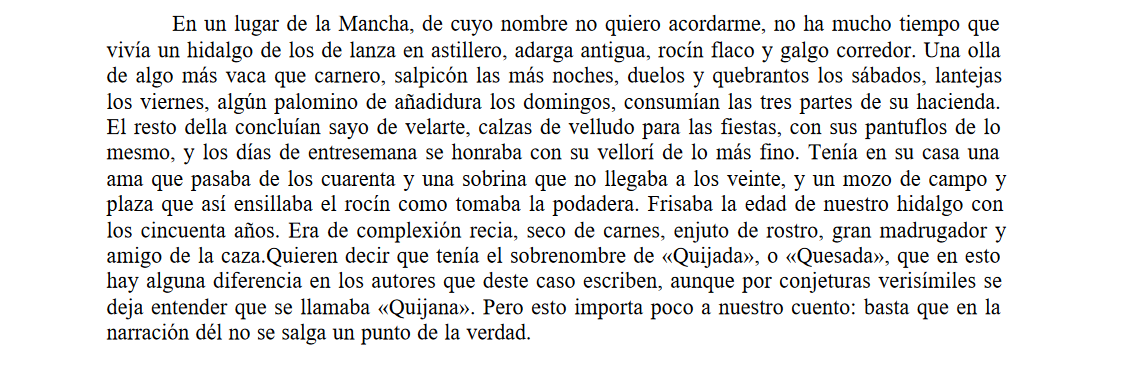
\includegraphics[width=1.15\textwidth]{Imagenes/Ejemplos/Cap1DonQuijote}
	\caption{Texto original de Don Quijote de la Mancha}
	\label{fig:Quijote}
\end{figure} 


\begin{figure}[htb]
	\centering
	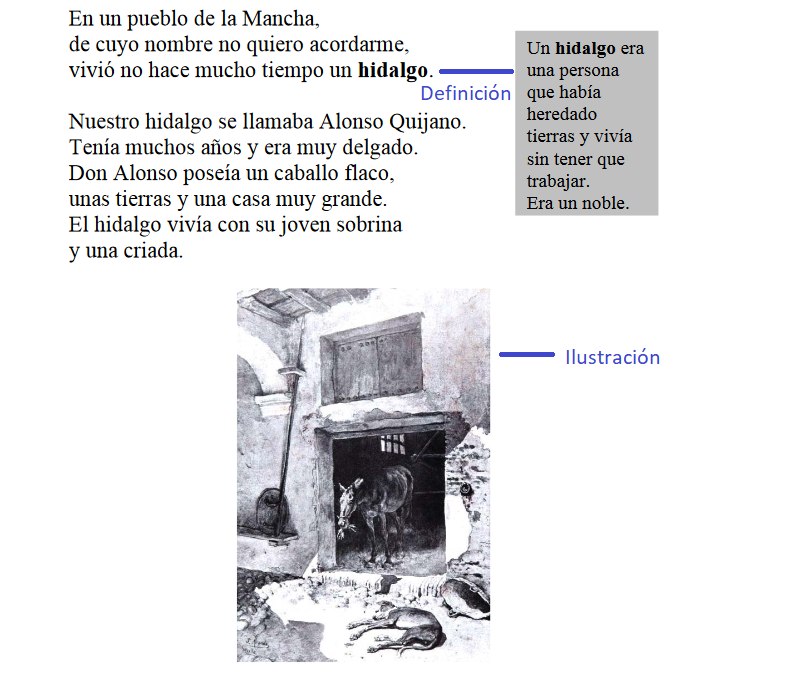
\includegraphics[width=0.7\textwidth]{Imagenes/Ejemplos/Cap1DonQuijoteLF}
	\caption{Texto LF de Don Quijote de la Mancha}
	\label{fig:QuijoteLF}
\end{figure}


\subsection{Un poco de Historia...}
El movimiento de la Lectura Fácil surgió en Suecia en 1968\footnote{https://www.lecturafacilextremadura.es/historia/}. En ese año se publicó el primer libro en Lectura Fácil y desde entonces hasta 1994 se crearon 330 obras, unas 15 y 20 nuevas cada año. Este movimiento se extiende a los países vecinos, Noruega y Finlandia.

En Noruega, por ejemplo, la iniciativa se denomina \textit{Leser s$\emptyset$ker bok”}\footnote{\href{https://lesersokerbok.no/english/}{Leser s$\emptyset$ker bok}} (Lector busca libro) y es una alianza de 20 organizaciones, que incluyen editoriales y organizaciones de personas con discapacidad.

En 1988, en Bruselas, se crea la organización \textit{Inclusion Europe}, la alianza europea de organizaciones que trabajan por los derechos de las personas con discapacidad, en la que se agrupa a organizaciones y asociaciones de personas con discapacidad intelectual de 40 países europeos e Israel.

En 1998, se elabora la guía \textit{«El camino más fácil: Directrices europeas para generar información de fácil lectura destinada a personas con discapacidad intelectual»\footnote{\href{http://www.lecturafacil.net/media/resources/ILSMHcastell\%C3\%A0.pdf}{http://www.lecturafacil.net/media/resources/ILSMHcastell\%C3\%A0.pdf}}} y se diseña un logotipo europeo de Lectura Fácil, para identificar todos los textos adaptados que siguen sus pautas.

En 2003, en España, se crea la primera Asociación de Lectura Fácil en Barcelona. Desde entonces, surgen diversas organizaciones e iniciativas a favor de la Lectura Fácil por toda España, donde hay más de 300 libros adaptados a LF para aquellas personas con problemas de lectura.

\subsection{Destinatarios de la LF}
La Lectura Fácil se dirige a una serie de grupos con ciertas dificultades de compresión lectora. Algunos de ellos son los siguientes: 
\begin{itemize}
	\item Personas con dificultades en el aprendizaje (como la dislexia, etc.)
	\item Personas con poca cultura o escasa escolarización.
	\item Personas extranjeras o inmigrantes que no dominan bien la lengua española.
	\item Niños que necesitan un refuerzo en la lectura.
	\item Personas sordas con dificultades en la comprensión.
	\item Personas mayores con trastornos mentales.
	\item Personas con hiperactividad y  déficit de atención. 
	\item Personas con discapacidad intelectual o del desarrollo (como el autismo, afasia, etc.). 
\end{itemize}


\subsection{¿Cómo se identifican los textos de LF?}
En los textos adaptados a Lectura Fácil vienen determinados por dos tipos de logotipos. En la figura \ref{fig:IFLA} es el logo que la Asociación de Lectura Fácil otorga a los textos que se adaptan a las normas de la Federación Internacional de Asociaciones de Bibliotecarios y Bibliotecas (IFLA), del inglés \textit{International Federation of Library Associations and Institutions}\footnote{\href{https://www.ifla.org/ES}{https://www.ifla.org/ES}}. Y la figura  \ref{fig:logoEuropeo}
Logo fomentado por Inclusion Europe \footnote{\href{http://www.inclusion-europe.eu/}{http://www.inclusion-europe.eu/}}.
\begin{figure}[htb]
\centering
	
\includegraphics[width=0.5\textwidth]{Imagenes/Logos/indice}
	\caption{Logo LF que cumplen las normas de la IFLA}
	\label{fig:IFLA}
\end{figure} 
\begin{figure}[htb]
	\centering
	
\includegraphics[width=0.3\textwidth]{Imagenes/Logos/indice2}
	\caption{Logotipo europeo de LF}
	\label{fig:logoEuropeo}
\end{figure} 




\subsection{Niveles de adaptación}
Es imposible adaptar un texto para todas las personas que necesiten este tipo de lectura.
 
La IFLA distingue entre los siguientes niveles de adaptación:
\begin{itemize}
	\item Primer nivel, es el más sencillo y simple con muchas imágenes y escaso texto, con una dificultas sintáctica baja.
\item Segundo nivel, es intermedio, menos sencillo que el anterior con un vocabulario y expresiones que son conocidas por todos, fácil de seguir y comprender e imágenes.
\item Tercer nivel, es el más complejo, con textos largos, palabras que no se conocen a menudo, con saltos en el tiempo y muy pocas imágenes. 
 \end{itemize}
\subsection{Pautas a seguir para la elaboración de Lectura Fácil}
 El primero documento de como elaborar texto adaptado a Lectura Fácil fue publicado por la IFLA. Hay otro que fue elaborado por varias organizaciones de Inclusion Europe bajo el título "Información para todos"\footnote{https://es.wikipedia.org/wiki/Lectura\_fácil\#Niveles} .
 
 Las pautas que se deben seguir se vincula a la ortografía, gramática, léxico, estilo, diseño, imágenes, formato, etc. 
 
 Algunos ejemplos y recomendaciones son las siguientes:
 \begin{itemize}
 \item Uso de frases simples, cortas y con una estructura habitual.
 \item Uso de imágenes sencillas y pictogramas de apoyo al texto, de manera descriptiva.
 \item Cada frase debe ocupar una línea. Si no es fuese posible deberá ocupar varias líneas.
 \item Evitar oraciones impersonales y pasivas reflejas.
 \item Evitar el subjuntivo o la voz pasiva.
 \item Evitar signos ortográficos poco habituales. (%, &, / ...)
 \item Evitar abreviaturas, acrónimos y siglas
 \item Uso de palabras de uso cotidiano y evitar tecnicismos.
 \item Ideas principales
 \item Redactar en modo directo
 \item No dar conocimientos previos por conocidos.
 \item Evitar diseños cargados.
  \item Eliminar información no necesaria.

\end{itemize}
\subsection{Movimientos y asociaciones}
Surgen una serie de movimientoscon el fin de integrar y favorecer a las personas con dificultades en la comprensión de lectura, la información y cultura a través de materiales de lectura adaptados. Algunos de ellos son los siguientes:
\begin{itemize}
	\item{\textbf{Asociación de Lectura Fácil de Barcelona}}\cite{LFBarcelona}. La asociación fue creada en 2003, la primera en España del movimiento LF. Es una asociación sin ánimo de lucro que trabaja para hacer fácil el acceso la lectura, cultura e información a todas las personas, en especial a aquellas con dificultades en la lectura. 
	
	\item{\textbf{Asociación Lectura Fácil Extremadura}}\cite{LFExtremadura}. Es una asociación sin ánimo de lucro que trabaja a favor de la promoción, implantación y difusión de la Fácil Lectura. Se encarga de  dar accesibilidad, inclusión, integración, participación y realización personal para distintos colectivos en situación de riesgo de exclusión económica y/o socio-cultural.
	
	\item{\textbf{Fundación Ciudadanía (Extremadura)}}\cite{LFFundacionCiudadania}. Fundación sin ánimo de lucro, declarada de Utilidad Pública,de carácter social que realiza aportaciones y estrategias en el ámbito de la Innovación Educativa y el Empleo, extendiendo su ámbito de actuación a todo el territorio español, poniendo énfasis en Extremadura y en su vocación europea y latinoamericana.
	
	\item{\textbf{Dilee Lectura Fácil (Extremadura)}}\cite{LFDilee}. Es una empresa española, pionera en Extremadura, que pretende implantar y consolidar la Lectura Fácil en todos los ámbitos y sectores de la vida económica, socio-política, artística-cultural, educativa, etc., en la comunidad extremeña.
	
	\item{\textbf{Lectura Fácil Madrid}}\cite{LFMadrid}. Es una asociación creada en el año 2013 que tienen como finalidad  lograr que todas las personas puedan participar de forma activa y responsable en la sociedad y hacer realidad la democracia lectora. 
	
	\item{\textbf{Cooperativa Altavoz (Madrid)}}\cite{LFCooperativaAltavoz}. Es una cooperativa formada por personas con discapacidad
	que trabaja para mejorar la autonomía de todas las personas, queriendo servir de modelo a personas como ellos.
	
	\item{\textbf{Lectura Fácil Euskadi (Bilbao)}}\cite{LFEuskadi}.Es una asociación que pretende incentivar la creación, difusión y utilización de materiales en Lectura Fácil, a través de un programa de animación a la lectura dirigido a personas con dificultad lectora.
	
	\item{\textbf{Lectura Fácil Castilla y León (Palencia)}}\cite{LFCastillaLeon}. Es una entidad sin ánimo de lucro que trabaja para difundir la Lectura Fácil como herramienta de conocimiento entre las personas con dificultades de comprensión lectora en Castilla y León.
	
	\item{\textbf{Instituto de Lectura Fácil (Sevilla)}}\cite{LFInstitutoSevilla}. Es una organización social con el objetivo de reivindicar el derecho que tenemos a comprender la información que nos rodea, dar calidad de vida a la ciudadanía, en especial de los colectivos más vulnerables de la sociedad.
	
		\item{\textbf{Plena Inclusión)}}\cite{PlenaInclusion}. Es una organización, formada por 17 federaciones autonómicas (Ceuta y Melilla también) y unas 900 asociaciones en toda España, que representa a las personas con discapacidad intelectual o del desarrollo.	Defienden los derechos y fomentan la calidad de vida de personas con discapacidad intelectual o del desarrollo y su familia. 
		
	\item{\textbf{diloFácil)}}\cite{DiloFacil}. Adaptan textos en Lectura Fácil para una comunicación más accesible.Han adaptado la Constitución española en Lectura Fácil
	
		\item{\textbf{SOLCOM}}\cite{SOLCOM}. Organización no gubernamental, independiente y orientada a dar asistencia legal para la solidaridad comunitaria de las personas con diversidad funcional y la inclusión social.
		
\end{itemize}

\subsection{Proyectos}
Asociaciones, movimientos o incluso grupos de personas han desarrollado desde el inicio de la creación de la LF hasta el día de hoy una serie de proyectos para poder ayudar a ese colectivo. 

Algunos son los siguientes:

\begin{itemize}
\item {\textbf{Dytective para dislexia}}, aplicación gratuita, desarrollada por Change Dyslexia, lo que pretende es mejorar la lectura y escritura con juegos, los cuales se personalizan para superarse día a día. Dirigido a niños con o sin dificultades en la lectura y la escritura. Su última actualización ha sido el 24 de marzo de 2020. 

Se puede descargar a través del siguiente enlace:

\href{https://www.changedyslexia.org/}{https://www.changedyslexia.org/}

\item {\textbf{Guía en Lectura Fácil sobre los servicios del banco}}, Plena inclusión Galicia ha publicado una guía en LF, el 21 de julio de 2020, sobre qué servicios te ofrece un banco y cómo manejar y administrar bien el dinero. 

Se puede ver y/o descargar a través del siguiente enlace:

\href{https://fademga.plenainclusiongalicia.org/dmdocuments/Los\_servicios\_del\_banco.pdf}{https://fademga.plenainclusiongalicia.org/dmdocuments/Los\_servicios\_del\_banco.pdf}


\item {\textbf{Léelo Fácil Educ. - Gallego}}, aplicación que sirve para leer un libro adaptado a lectura fácil con dibujos, música y animaciones para que se entienda mejor. Esta aplicación es gracias a LÉELO FÁCIL, proyecto de FEAPS (Confederación Española de Organizaciones en
favor de las Personas con Discapacidad Intelectual), que actualmente, desde octubre de 2015, se trata de Plena Inclusión. Su fecha de publicación fue el 13 de marzo del 2015 y no ha habido actualizaciones posteriores. 

Se puede descargar a través del siguiente enlace:

\href{https://apkpure.com/es/l\%C3\%A9elo-f\%C3\%A1cil-educ-gallego/com.oneclick.ga.rayoluna}{https://apkpure.com/es/l\%C3\%A9elo-f\%C3\%A1cil-educ-gallego/com.oneclick.ga.rayolun}

\item
{\textbf{Guía de uso del Metro de Madrid en Lectura fácil}}, en esta guía adaptada a LF, que tiene como objetivo contribuir a que las personas con discapacidad intelectual puedan moverse por la red del suburbano de forma autónoma. Fue publicada por Plena Inclusión en el año 2019 y ha sido revisada y actualizada en 2020. 

Se puede ver y/o descargar a través del siguiente enlace:


\href{https://plenainclusionmadrid.org/wp-content/uploads/2020/06/Gu\%C3\%ADa-de-uso-de-Metro-en-lectura-f\%C3\%A1cil.pdf}{https://plenainclusionmadrid.org/wp-content/uploads/2020/06/Gu\%C3\%ADa-de-uso-de-Metro-en-lectura-f\%C3\%A1cil.pdf}

\item
{\textbf{Guía del Museo del Prado}}, el Museo del Prado, en colaboración con Plena Inclusión Madrid, publica su primera guía en lectura fácil el 20 de febrero del 2020, el Museo del Prado ha publicado una guía en lectura fácil, que ofrece información sobre 10 obras maestras del museo.

\href{https://content3.cdnprado.net/doclinks/pdf/visita/plano/accesible/Guia\_accesible\_MNP.pdf}{https://content3.cdnprado.net/doclinks/pdf/visita/plano/accesible/Guia\_accesible\_MNP.pdf}


\item
{\textbf{Noticias Fácil}}, proyecto de Discapnet que se creó en el marco del Plan Avanza del Ministerio de Industria, Comercio y Turismo de España. Es una plataforma con contenidos web adaptados a LF relacionados con la actualidad. 

Se puede acceder a su página a través del siguiente enlace:

\href{http://www.noticiasfacil.es/}{http://www.noticiasfacil.es/}

\item
{\textbf{Simplext}}, sistema automático de transformación de contenidos de textos de fácil lectura, proyecto de Investigación Industrial parcialmente financiado por el Ministerio de Industria, Turismo y Comercio mediante el Plan Nacional de Investigación Científica, Desarrollo e Innovación Tecnológica (I+D+i). Es un producto para la simplificación automática de textos en español para que su lectura resulte más comprensible a aquellas personas con dificultades cognitivas. En la 10ª edición de los premios BDigital a la Innovación Digital fue nominado y finalista.

Se puede acceder a través del siguiente enlace:
 
\href{http://simplext.taln.upf.edu/}{http://simplext.taln.upf.edu/}

\item
{\textbf{Able to Include}}, proyecto Europeo de investigación, pretende facilitar la integración de personas con discapacidad intelectual, apoyado en aplicaciones con nuevas tecnologías en las áreas de ocio, movilidad e integración laboral. Proyecto creado en septiembre del 2013.

Se puede acceder a través del siguiente enlace:

\href{http://able-to-include.com/}{http://able-to-include.com/}

\item
{\textbf{Proyecto de Lectura Fácil sobre COVID-19}}, un documento sobre el COVID-19 adaptado a LF, publicado el 4 de noviembre de 2020, elaborado con la colaboración entre la Clínica Universidad de los Andes, y la casa de estudios, para que personas con discapacidad cognitiva, puedan comprender de manera más fácil acerca de la nueva enfermedad.

Se puede ver y/o descargar a través del siguiente enlace:

\href{https://www.clinicauandes.cl/docs/default-source/boletines/informaci\%C3\%B3n-coronavirus-en-lf.pdf?sfvrsn=199472df\_2}{https://www.clinicauandes.cl/docs/default-source/boletines/informaci\%C3\%B3n-coronavirus-en-lf.pdf?sfvrsn=199472df\_2}

\item
{\textbf{"Frente al aislamiento. Nos conectamos"}}, plena Inclusión desarrolla una aplicación, en marzo del 2020, que ofrece documentos, foros de consulta para preguntar dudas y agenda de actividades. Es una app gratuita para móviles android e IOS. 

Se puede descargar a través del siguiente enlace:

\href{https://my.yapp.us/ZNMC4A}{https://my.yapp.us/ZNMC4A}

\item
{\textbf{CAPITO}}, herramienta para adaptar textos a diferentes niveles del idioma

\item
{\textbf{SIMPATICO}}, proyecto europeo de investigación e innovación que trata de simplificar la interacción con la Administración Pública a través de las tecnologías para ciudadanos y empresas, es decir, mejorar la experiencia en las interacciones con los servicios electrónicos basados en tecnologías avanzadas de sistemas cognitivos. 

Más información en el siguiente enlace:


\href{https://dh.fbk.eu/2016/06/simpatico-h2020-project/}{https://dh.fbk.eu/2016/06/simpatico-h2020-project/}

\item
{\textbf{FIRST}}, una herramienta de adaptación de texto semiautomática para inglés, español y búlgaro para mejorar la accesibilidad de los textos escritos a personas con autismo. Proyecto psicolingüístico con técnicas de Inteligencia Artificial (IA).

\item
{\textbf{Comunicación Clara}}, el objetivo es facilitar el diálogo con los ciudadanos y los clientes de una forma sencilla y transparente. Es un asistente virtual que se aplica a cualquier tipo de documento, que valora la claridad del texto bajo 9 criterios. La valoración se da con una explicación de los motivos y consejos para mejorar el texto. Desarrollado por la empresa Prodigioso Volcán, en colaboración con el Instituto de Ingeniería del Conocimiento (IIC).

Más información:

\href{https://comunicacionclara.com/}{https://comunicacionclara.com/}



\end{itemize}




%En el estado de la cuestión es donde aparecen gran parte de las referencias bibliográficas del trabajo. Una de las formas más cómodas de gestionar la bibliografía en {\LaTeX} es utilizando \textbf{bibtex}. Las entradas bibliográficas deben estar en un fichero con extensión \textit{.bib} (con esta plantilla se proporcionan 3, dos de los cuales están vacíos). Cada entrada bibliográfica tiene una clave que permite referenciarla desde cualquier parte del texto con los siguiente comandos:

%\begin{itemize}
%\item Referencia bibliografica con cite: \cite{ldesc2e}
%\item Referencia bibliográfica con citep: \citep{notsoshort}
%\item Referencia bibliográfica con citet: \citet{latexAPrimer}
%\end{itemize}

%Es posible citar más de una fuente, como por ejemplo %\citep{latexCompanion,LaTeXLamport,texKnuth}

%Después, latex se ocupa de rellenar la sección de bibliografía con las entradas \textbf{que hayan sido citadas} (es decir, no con todas las entradas que hay en el .bib, sino sólo con aquellas que se hayan citado en alguna parte del texto).

%Bibtex es un programa separado de latex, pdflatex o cualquier otra cosa que se use para compilar los .tex, de manera que para que se rellene correctamente la sección de bibliografía es necesario compilar primero el trabajo (a veces es necesario compilarlo dos veces), compilar después con bibtex, y volver a compilar otra vez el trabajo (de nuevo, puede ser necesario compilarlo dos veces). 
